\documentclass[uplatex,dvipdfmx]{jsarticle}

\usepackage[uplatex,deluxe]{otf} % UTF
\usepackage[noalphabet]{pxchfon} % must be after otf package
\usepackage{stix2} %欧文＆数式フォント
\usepackage[fleqn,tbtags]{mathtools} % 数式関連 (w/ amsmath)
\usepackage{amsmath}
\usepackage{mathtools}
\usepackage{hira-stix} % ヒラギノフォント＆STIX2 フォント代替定義（Warning回避）
\usepackage{titlesec} % セクションのフォント変更用
\usepackage{listings} 
\usepackage{url}
\lstset{
basicstyle={\ttfamily}, 
identifierstyle={\small}, 
commentstyle={\smallitshape}, 
keywordstyle={\small\bfseries},  
ndkeywordstyle={\small},  
stringstyle={\small\ttfamily},  
frame={tb},  breaklines=true,  
columns=[l]{fullflexible},  
numbers=left,  xrightmargin=0zw,  xleftmargin=3zw,  
numberstyle={\scriptsize},  stepnumber=1, 
numbersep=1zw,  lineskip=-0.5ex
}

\titleformat*{\section}{\rmfamily\mcfamily\Large} % \sectionのフォントを明朝体に設定
\titleformat*{\subsection}{\rmfamily\mcfamily\Large} 
\titleformat*{\subsubsection}{\rmfamily\mcfamily\Large} 

\begin{document}
\title{数理モデリング 第6回レポート課題}
\author{学籍番号: 24G1122\\氏名: 細澤悠真}
\date{\today}
\maketitle

\section{課題3}
課題3：改良したSIRを解くプログラムを作成し、予測通り動いたか、動かなかったかなどを検討せよ。
\subsection{改良した内容}
SIRモデルに死亡者数の要素を加えたSIRモデルを作成した。この改良したSIRモデルでは、感染者数から回復者数に移る割合に加えて、死亡者数に移る割合を設定することができる。これにより、感染症の流行に伴う死亡者数の増加を考慮することができる。また、総人口数から死亡者数を差し引いて、人口に流動性を持たせた。
\subsection{予測した内容}
死亡者数を追加したことで、SIRモデルのS：感受性人口、I：感染者数、R：回復者数、D：死亡者数のそれぞれ4つの要素が時間の経過に伴い、減少傾向になると予測した。また、感染者数のピークがSIRモデルよりも低くなり、感染症の流行が緩やかになると予測した。
\subsection{結果と考察}
以下に、改良したSIRモデルによって、シミュレーションを行った結果を示す。
\begin{figure}[h]
    \centering
    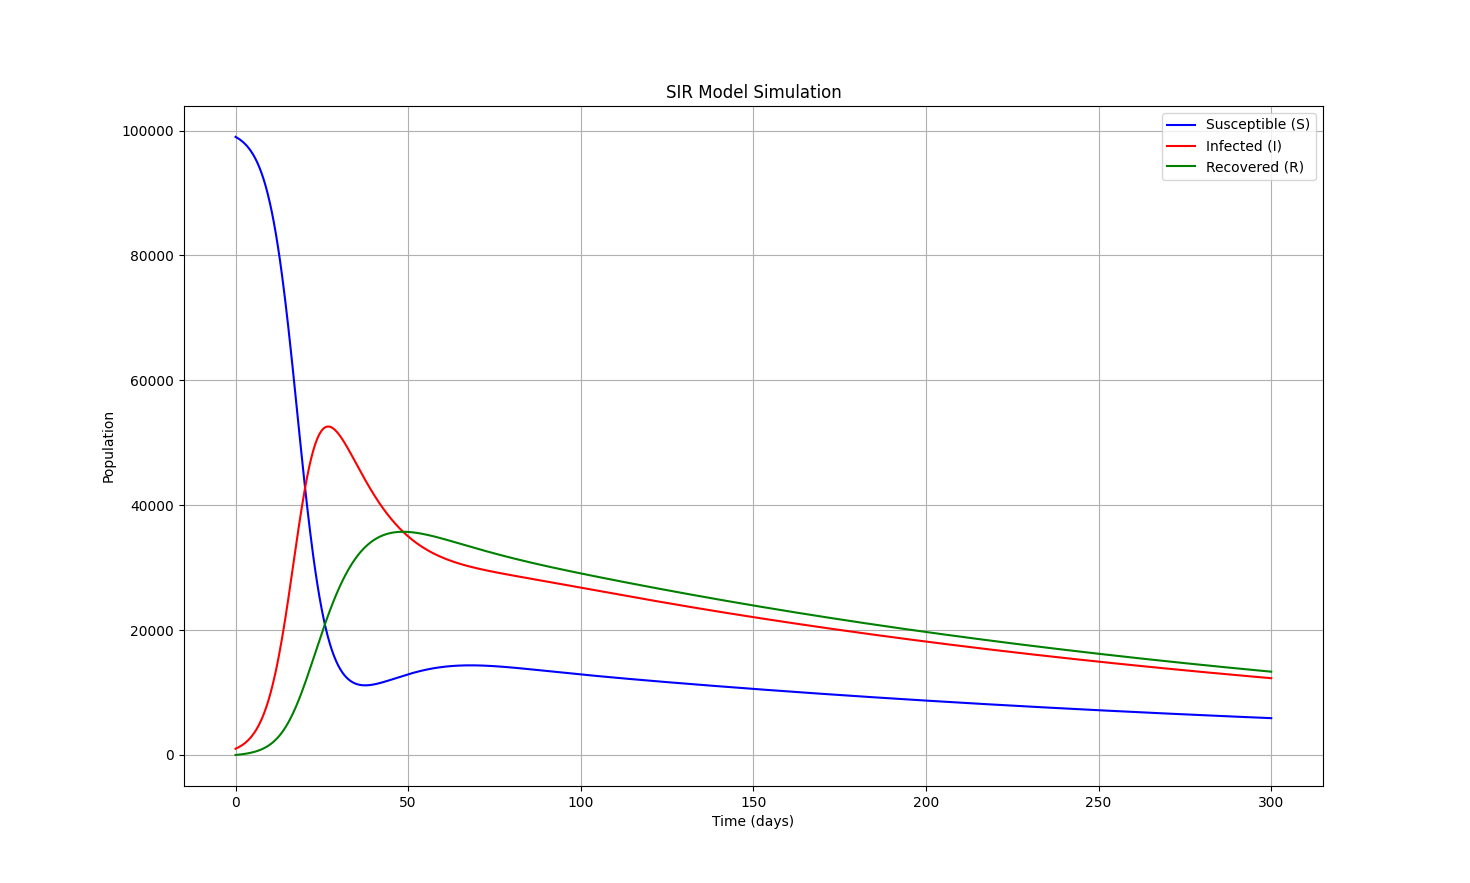
\includegraphics[width=0.8\textwidth]{assign8-3.png}
    \caption{改良したSIRモデルのシミュレーション結果}
    \label{fig:assign8-3}
\end{figure}
\newpage
図\ref{fig:assign8-3}より、感染者数、回復者数、死亡者数のそれぞれが時間の経過に伴い減少傾向になることが確認できた。これは、感染症の流行に伴い、死亡者数が増加することで、総人口数が減少し、感受性人口が減少するためである。
また、感染者数のピークがSIRモデルよりも低くなり、感染症の流行が緩やかになることも確認できた。これは、死亡者数の増加により、感染者数が減少するためである。以上の結果から、改良したSIRモデルは予測通りに動作し、感染症の流行に伴う死亡者数の増加を考慮することができることが示された。
\end{document}